\chapter{Fundamentação Teórica}
\label{cap:fundamentacao-teorica}

Corresponde à ``revisão de literatura'' ou ``marco teórico'' do Guia UECE 2026 (2.2.3.3, item a). Aqui você situa o leitor no estado da arte: cite os trabalhos e autores relacionados ao seu tema, apresentando as informações básicas necessárias para o entendimento do problema pesquisado, reforçando a necessidade do seu estudo e preparando o terreno para a interpretação dos resultados que virão mais adiante.

Duas regras não são automáticas e exigem atenção do autor:

\begin{alineas}
	\item todo autor citado nesta e nas demais seções precisa constar nas Referências, e todo autor que consta nas Referências precisa ter sido efetivamente citado no texto -- a lista bibliográfica não é um repositório de leituras, é um espelho exato das citações feitas;
	\item se a revisão de literatura for breve, ela pode ser dispensada como capítulo próprio e incorporada à Introdução -- a escolha fica a critério do autor ou da orientação.
\end{alineas}

Divida este capítulo em quantas seções fizerem sentido para o seu tema (uma por eixo teórico, por exemplo), substituindo as seções de exemplo abaixo.

\section{Fundamentação Teórica A}
\label{sec:fundamentacao-teorica-a}

Escreva aqui a discussão teórica relativa ao seu primeiro eixo temático, sempre apoiada em citação de autores -- por exemplo, \cite{lamport1986latex}, no sistema autor-data adotado neste template.

Os blocos abaixo demonstram, a título de exemplo, a sintaxe para inserir uma figura e uma tabela no texto -- mantenha-os como referência de uso e substitua apenas o conteúdo (imagem, legenda e fonte) quando for inserir as suas próprias ilustrações. Conforme o Guia (2.3.10-2.3.11), toda ilustração e toda tabela devem ter identificação numérica sequencial, legenda breve e a indicação obrigatória da fonte -- mesmo quando produzida pelo próprio autor, hipótese em que se escreve ``Elaborado pelo autor''.

	\begin{figure}[ht!]
		\centering
		\Caption{\label{fig:exemplo-1} Exemplo de figura inserida no texto, com legenda breve e autoexplicativa}
		\UECEfig{}{
			\fbox{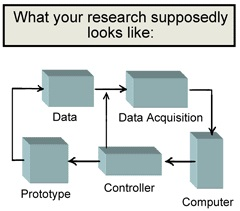
\includegraphics[width=8cm]{figuras/figura-1}}
		}{
			\Fonte{Elaborado pelo autor}
		}
	\end{figure}

As ilustrações devem ser inseridas o mais próximo possível do trecho do texto a que se referem, e o texto deve comentá-las (não basta inserir a figura -- explique o que ela mostra e por que ela importa para o argumento).

\section{Fundamentação Teórica B}
\label{sec:fundamentacao-teorica-b}

Escreva aqui a discussão teórica relativa ao seu segundo eixo temático. Ao final desta seção, é comum inserir um quadro-síntese comparando autores, conceitos ou abordagens.

	\begin{table}[ht!]
		\centering
		\Caption{\label{tab:exemplo-1} Exemplo de tabela com dados numéricos comparativos entre os autores/abordagens discutidos}
		\UECEtab{}{
			\begin{tabular}{cll}
				\toprule
				Critério & Abordagem 1 & Abordagem 2 \\
				\midrule \midrule
				Vantagem principal & Descreva aqui & Descreva aqui\\
				Limitação principal & Descreva aqui & Descreva aqui\\
				\bottomrule
			\end{tabular}
		}{
		\Fonte{Elaborado pelo autor}
	}
	\end{table}

Ao encerrar o capítulo, é útil fechar com um parágrafo de síntese que amarre os eixos discutidos e prepare a transição para o capítulo seguinte (Trabalhos Relacionados ou Metodologia, conforme a estrutura do seu trabalho).

O exemplo a seguir demonstra o uso de alíneas e subalíneas (Guia 2.3.6.1-2.3.6.2: recuo de 2 cm para alíneas e 2,5 cm para subalíneas), úteis quando você precisar enumerar itens dentro de um parágrafo:

\begin{alineascomponto}
	\item Substitua por um primeiro ponto da sua síntese
	\item Substitua por um segundo ponto da sua síntese
	\item Substitua por um terceiro ponto, desdobrado em subalíneas
	\begin{subalineascomponto}
		\item Primeiro desdobramento
		\item Segundo desdobramento
	\end{subalineascomponto}
\end{alineascomponto}
